\documentclass[a4paper]{article}
\usepackage[letterpaper, margin=1in]{geometry} % page format
\usepackage{listings} % this package is for including code
\usepackage{graphicx} % this package is for including figures
\usepackage{amsmath}  % this package is for math and matrices
\usepackage{amsfonts} % this package is for math fonts
\usepackage{tikz} % for drawings
\usepackage{hyperref} % for urls

\title{Project Proposal}
\author{Sami Ellougani and Brian Henderson}
\date{9/23/17}

\begin{document}
\lstset{language=Python}

\maketitle

\section{Proposal}
Our semester project is to implement deep neural networks for artistic style transfer. To achieve this we will be using convolution neural networks to
train styles. We've decided to apply the style transfer in real time, which will involve training networks with a designated style. [1] We will
use the resource below as a guide to how the TensorFlow implementation. Our objective is for a user to be able to upload an image, select a preloaded style, and produce
the output. Once the training algorithim is optimized, we will continue to upload various influential, abstract, and unique styles from different historical and modern
time periods. 


\section{Datasets}
The Dataset that we are going to utilize the most is the Microsoft Coco dataset. The Microsoft Coco dataset is mainly utilized for 
Object segmentation, recognition in context, and captionining. The Coco dataset consists of of 330,000 images, 1.5 million object instances, 
80 object categories, and 5 captions per image.

\section{Training}
Training involves evaluating the loss for a given training/testing example, and then utilizing this error within each layer of our network. 
At each layer, we compute the gradient descent of the layer's weight with the error margin, and use this to make changes to the weights in a negative 
direction of the gradient. This is known as gradient descent via backpropagation.

\section{Sources}
\href{https://shafeentejani.github.io/2017-01-03/fast-style-transfer/}{Main Source} \\
	1  https://shafeentejani.github.io/2017-01-03/fast-style-transfer/

\section{Example Output}
\begin{figure}
  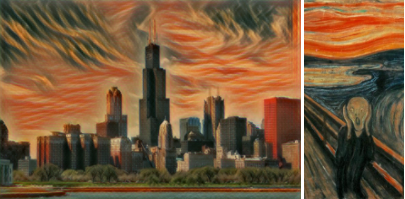
\includegraphics[width=75mm]{example.png}
\end{figure}

\end{document}